\chapter{``Quantum" Behavior}
\label{Ch1}

\section{Oil Droplet System}
	    \label{parameters}
	       Consider a fluid of density $\rho$, viscosity $\nu$, and surface tension $\sigma$ in a bath of depth $H$. This fluid bath is then driven vertically at an amplitude $A_0$ at frequency $f=\omega/{2\pi}$. By defining $\mathnormal{\gamma}=A_0\omega^2$, the effective gravity in the frame of reference of the bath is $g+\gamma~\mathrm{sin}(\omega t)$. The surface of oil in the shaking tray remains quiescent for lower values of $\gamma$. However, if one continues to increase $\gamma$ (by increasing $A_0$ or $f$), one will eventually witness the appearance of standing surface waves called Faraday waves. We define the threshold at which these waves appear as the Faraday threshold $\gamma_\mathrm{F}$, the value of which changes depending on the size and shape of the tray, the amount of fluid in the tray, and the properties of the fluid. 
	       
	   \begin{figure}[h]
	       \centering
	    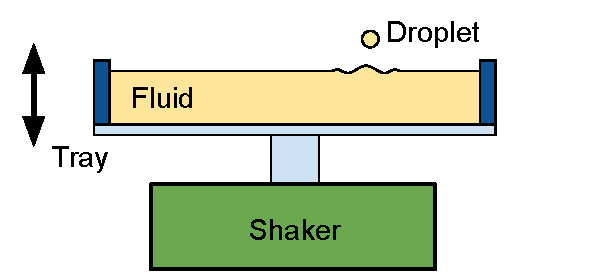
\includegraphics[scale=.80]{basicsetup.pdf}
	     \caption{A droplet bounces on a vertically vibrating fluid bath. The tray vibrates with an amplitude $A_0$ at frequency $f$.}
	 \label{regime}
	\end{figure}
	       
	    If we take a toothpick and break the surface of the vibrating oil bath, we form a droplet of oil that will remain bouncing for hours. The oil droplet of diameter $D$ bounces when for specific values of $\gamma$. For a small $\gamma$, the forcing is not enough to sustain the droplet, and it quickly coalesces. Increasing $\gamma$ will eventually reveal a region in which standing surface waves cover the entire tray. These waves are called Faraday waves, and the acceleration at which they first appear is referred to as the Faraday threshold $\gamma_\mathrm{F}$, which varies depending on the amount, density, and viscosity of fluid. The range of the various parameters which allow for the existence of the bouncing droplet are outlined in \refTab{approxlimits}. 
	      
	       \begin{table}[htdp] 
\caption[Basic Table 1]{Approximate limits for bouncing drop behavior. The value $g = 9.81\mathrm{ms}^{-2}$ is the standard acceleration due to gravity.} 
\begin{center} 
\begin{tabular}{c c c} 
\toprule 
  Parameter &  Lower Limit & Upper Limit \\
  \midrule
Viscocity $\nu$ (cSt) & 10 & 100 \\ 
Bath Depth $H$ (mm) & 4 & 10 \\
Frequency $f$ (Hz) & 20 & 150 \\
Amplitude $A_0$ (mm) & 0.1 & 1 \\
Drop Diameter $D$ (mm) & 0.6 & 1.0 \\
Forcing Acceleration $\gamma$ ($\mathrm{ms}^{-2}$) & 0.5$g$ & $\gamma_\mathrm{F} \approx 4.2g$ \\
\bottomrule 
\end{tabular}
\end{center}
\label{approxlimits} 
\end{table}	

\subsection{Faraday Waves}
	       At a forcing $\gamma = \gamma_\mathrm{F}$ we see the appearance of standing surface waves known as Faraday waves. These waves have frequency $f_\mathrm{F} = f/2$ and a angular frequency $\omega_\mathrm{F} = 2\pi f_\mathrm{F}=\pi f$. The standing wave and water dispersion relation can be used to find the wavelengths of standing waves at the Faraday threshold:
\begin{equation} \label{dispersion}
\omega_\mathrm{F}^2 = \left(gk_\mathrm{F}+\frac{\sigma k_\mathrm{F}^3}{\rho}\right)\mathrm{tanh}(k_\mathrm{F}H),
\end{equation} 
which relates the angular Faraday frequency $\omega_\mathrm{F}$ to the Faraday wavenumber $k_\mathrm{F}$ \rf{Kumar}. From the wavenumber, we can calculate the wavelength $\lambda_\mathrm{F}$ of the Faraday waves by the relation $\lambda_\mathrm{F}$ = $2\pi/k_\mathrm{F}$. Though we are interested in investigating the region $\gamma < \gamma_\mathrm{F}$ where there are no standing surface waves, \refeq{dispersion} provides an estimate to the wavelength and frequency of waves in the bouncing droplet system. 


\subsection{Vibration Number}

In an experiment, one usually pours in a specific volume of oil in the tray, fixing the values of $\nu$, $\sigma$, and $H$. One is then left with the option to adjust $\gamma$ which produces a range of droplet motions, including a slew of different stationary bouncing modes and linear or chaotic ``walking" trajectories. To visualize the various bounving behaviors, we use the vibration number $V_i$, which takes into account many of the parameters of the experiment \rf{Molacek2013}. The vibration number is the ratio of the forcing frequency and the drop's natural oscillation frequency:
\begin{equation} \label{vibrationnumber1}
V_i = \frac{\omega}{\omega_\mathrm{D}}
\end{equation}   
where $\omega_\mathrm{D}$ represents the oscillation frequency of a fluid droplet. In other words, it represents ...!!! The oscillation frequency of a fluid droplet is defined as:
\begin{equation} \label{oscillationfrequency}
\omega_\mathrm{D} = 2\sqrt{\frac{2\sigma}{\rho D^3}},
\end{equation}   
with surface tension $\sigma$, density $\rho$ , and diameter of the droplet $D$ \rf{lord}. Combining \refeqs{vibrationnumber1}{oscillationfrequency} we arrive at:
\begin{equation} \label{vibrationnumber2}
V_i = \frac{\omega}{2}\sqrt{\frac{\rho D^3}{2\sigma}},
\end{equation}   	       	       
a dimensionless parameter that captures the fluid's surface tension $\sigma$ and density$\rho$, the tray's vibration $\omega$, and the droplet's diameter $D$. The natural frequency of the droplet occurs around $V_i \approx 0.65$, where the droplet can exhibit both walking and bouncing behaviors. Setting up a plot with $V_i$ on the y axis and (dimensionless) ${\gamma}/{g}$ on the x axis allows the experimenter to identify regions of similar behaviors, shown in \refFig{regime}. If we hold the fluid and the frequency constant ($\sigma$, $\rho$, and $\omega$), then we can think of increasing $V_i$ as and increasing droplet diameter $D$. 
	    
	    \begin{figure}[h]
	% the options are h = here, t = top, b = bottom, p = page of figures.
	% you can add an exclamation mark to make it try harder, and multiple
	% options if you have an order of preference, e.g.
	% \begin{figure}[h!tbp]
	       \centering
	    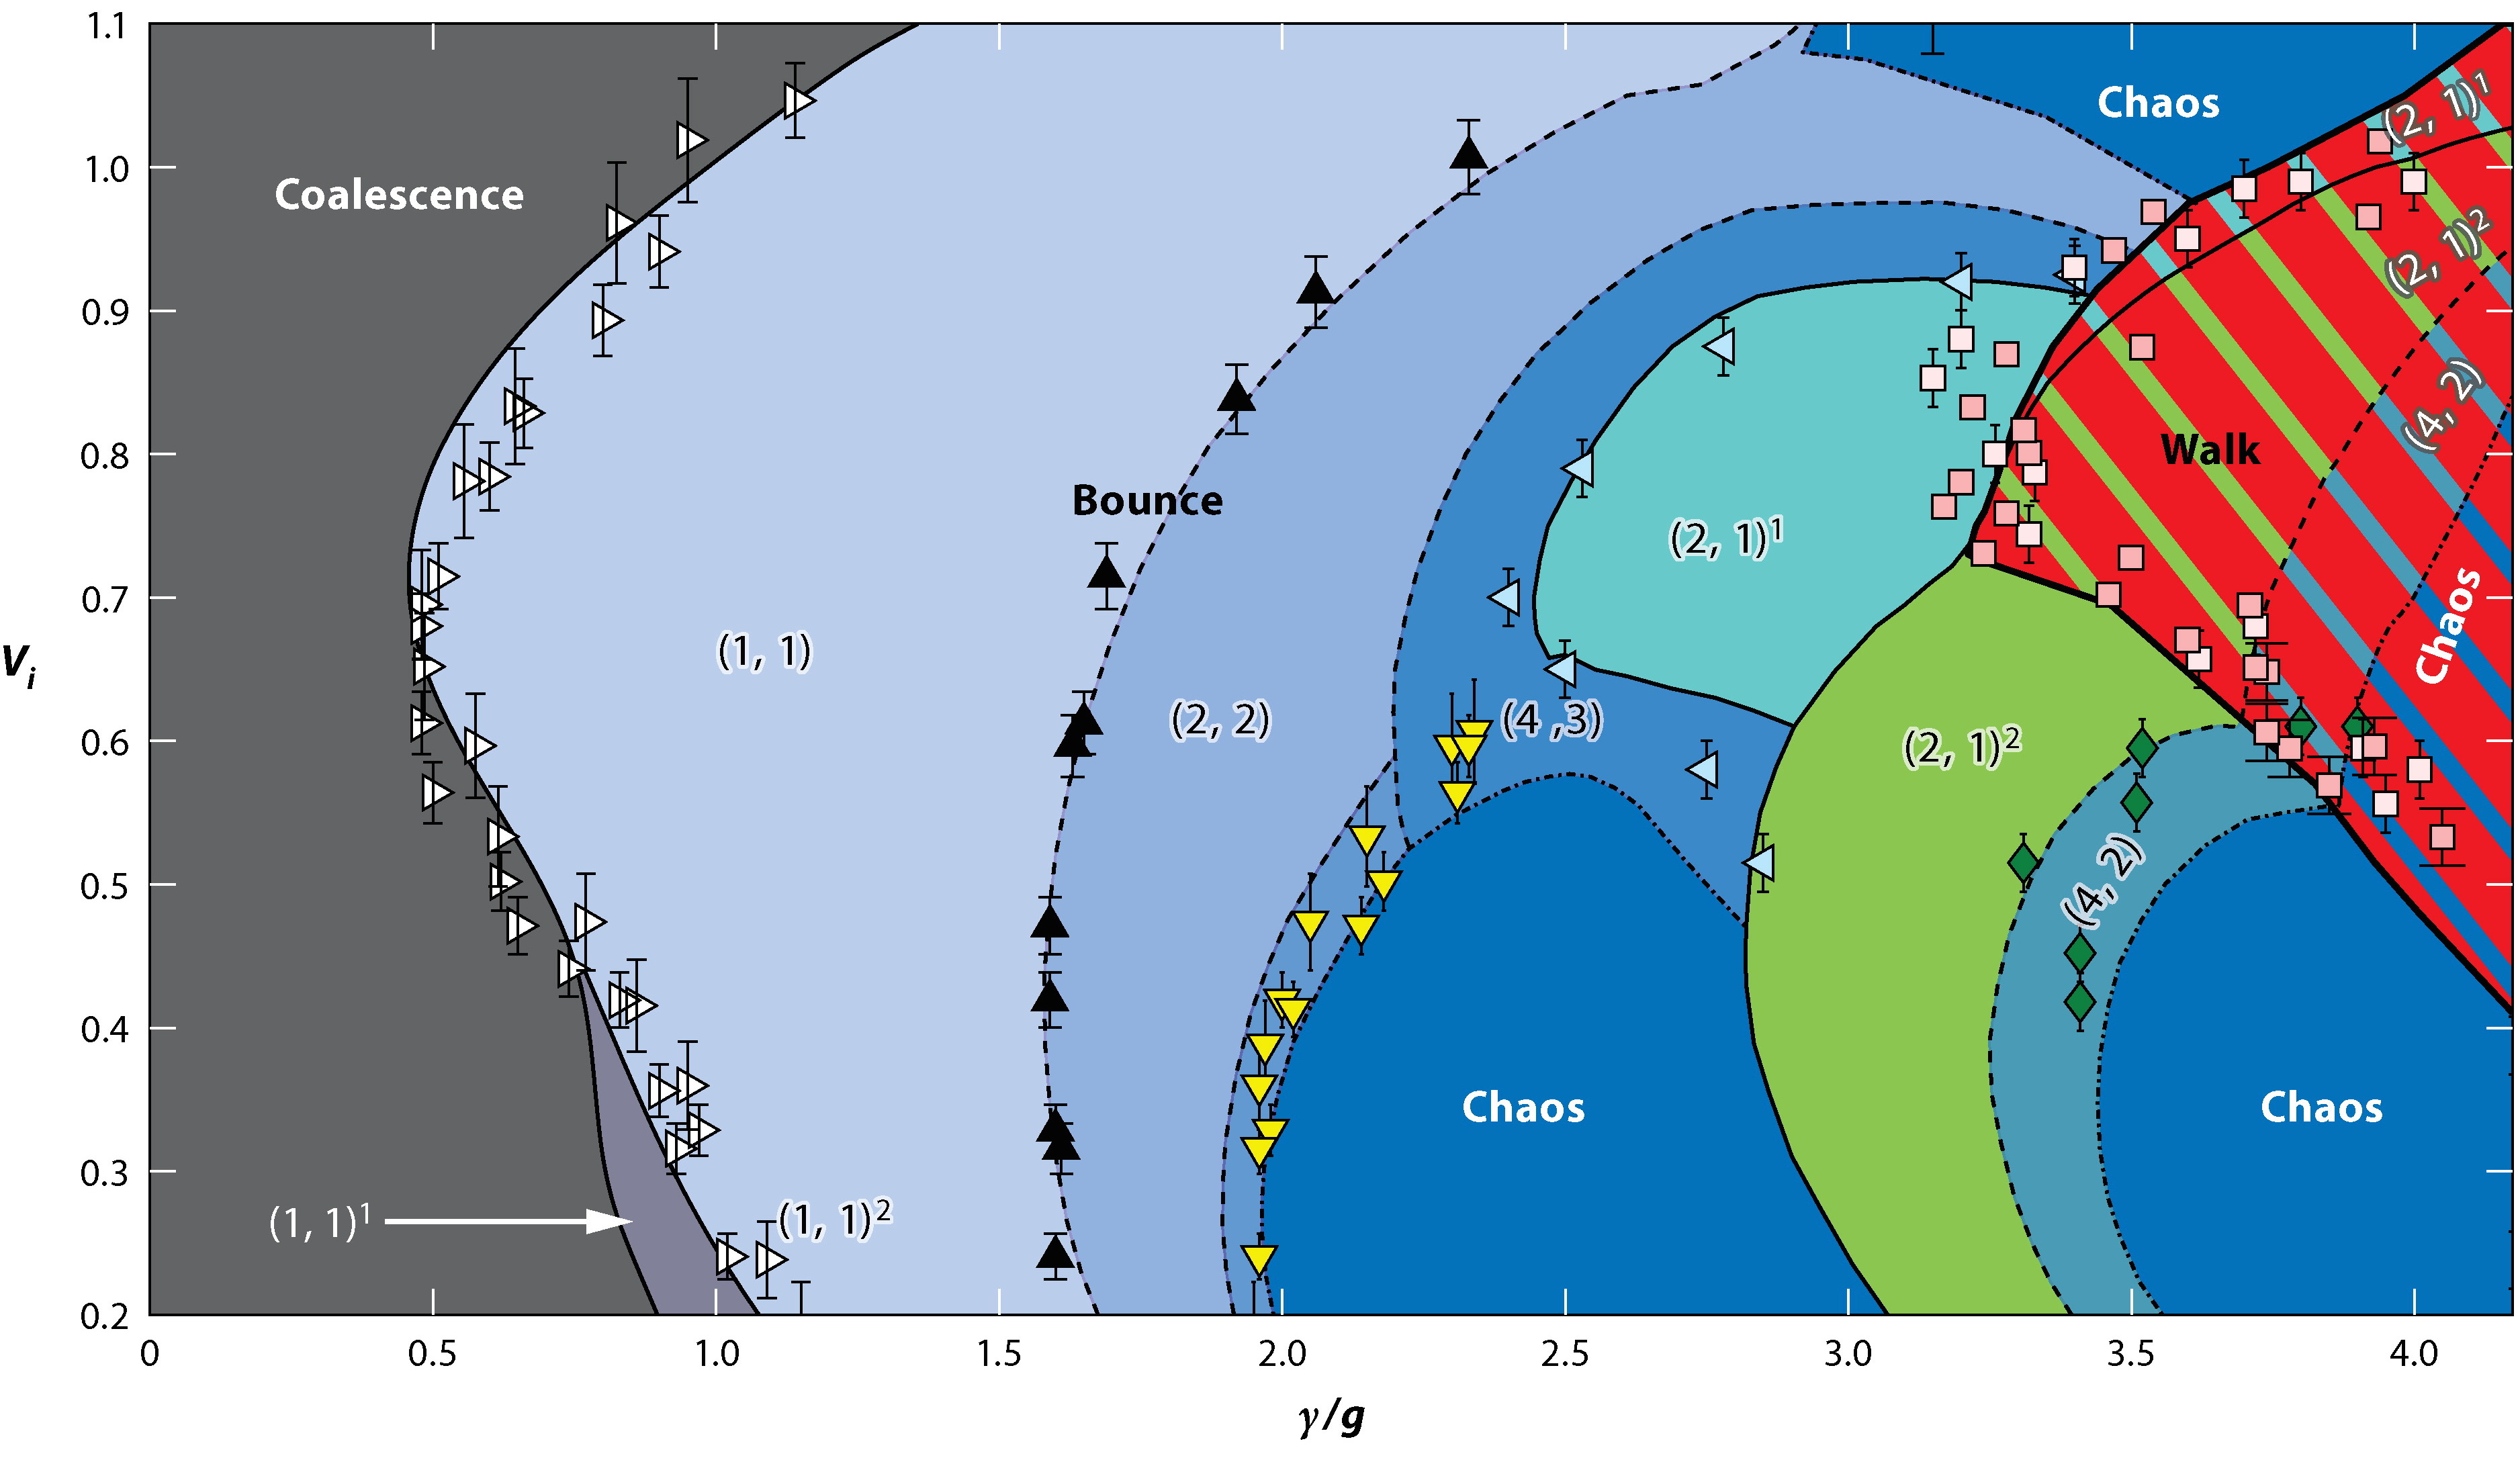
\includegraphics[scale=.96]{vibrationnumber}
	     \caption{The different bouncing regimes for the oil drops of 20 cSt silicone oil at $f$ = $\omega / 2\pi$ = 80 Hz, characterized by the non-dimensionalized forcing frequency $\gamma/g$ and the vibration number $V_i$. The parameters $(m,n)^{i}$ describe a droplet that bounces $n$ times in $m$ forcing periods, where $i$ distinguishes modes with different mechanical energy. The Faraday threshold is $\gamma_\mathrm{F} = 4.2$. This diagram was taken from \rf{pilot-wave}.}
	 \label{regime}
	\end{figure}

The various modes seen in \refFig{regime} can be described by ($m$,$n$), where $n$ is the number to times the droplet contacts the surface over period $m/f$. For example, in the (1,1) ``Bounce" mode, the droplet hits the oil bath once per up-and-down motion of the tray. In the (2,2) mode, the drop makes two bounces of differing heights. The ``Chaos" regimes indicate that the bouncing of the droplet is chaotic, and it does not seem to exhibit a periodic bouncing motion. The ``Walk" regime describes a very particular kind of behavior in which the droplet moves forward as it bounces, seemingly walking across the surface. Like bouncing, walking also comes in various modes. Finally, the ``Coalescence" region demarcates the coalesces of the droplet with the bath.

The droplet map shown in \refFig{regime} provides a valuable starting place for an experiment since it outlines the many possible states of the system. We will now narrow our focus to only the walking regime, for which a variety of fascinating interactions emerge.

	                   \subsection{Walking}
            
            
            
             \begin{figure}[h]
	       \centering
	    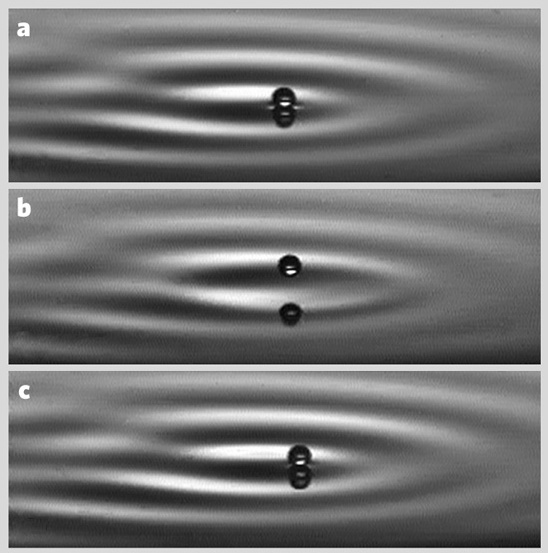
\includegraphics[scale=.6]{CouderWalkers.jpg}
	     \caption{The series of pictures (a) - (c) show a droplet bouncing off of the slope of the localized wave, launching into the air, and then falling again on a new wave slope. This periodic process happens multiple times per second, giving the droplet the appearance of walking across the surface. Figure adapted from \rf{Couder2005b}.}
	 \label{Couderwalkers}
	\end{figure}


            \subsection{Path Memory}
                        
            Path memory is a parameter that can be varied in this setup; essentially it captures the importance of damping in the system \rf{Eddi2011}. Every time the droplet impacts the bath, it creates a radial traveling wave. Over the course of many bounces, a guiding wave field composed of a superposition of the many waves arises. In this way the wave field ``remembers" previous interactions, but is at the same time being periodically ``updated" with every new bounce of the droplet. Because droplet motion is influenced by the wave field, controlling the damping of the wave field will influence the path of the walker. 
            
For a bouncing droplet in which the guiding waves decay relatively quickly, the droplet can only be influenced by relatively recent waves. This kind of behavior is characterized as a low memory. Conversely, a high memory system is one in which waves do not decay quickly; they propagate outwards and reflect off of the surfaces of the tray before reflecting back and interfering with the other waves produced by the droplet. As one gets closer to the Faraday threshold, one achieves higher and higher memory because waves last for longer. The quantum-like features of this experiment arise in the high-memory limit. 

The non-dimensional memory parameter is formally defined as:
$$M_e = \frac{T_\mathrm{d}}{T_\mathrm{F}(1-\gamma/\gamma_\mathrm{F})},$$
where $T_\mathrm{d}$ is the decay time of waves in the absence of vibration and $T_\mathrm{F}$ is the period of the Faraday waves \rf{Harris2013}. It will suffice to discuss memory as a fraction of the Faraday threshold $\gamma/\gamma_{F}$, since the fraction and $M_e$ are monotonically related. As the value of $\gamma/\gamma_{F}$ increases (we get closer to the Faraday threshold), $M_e$ increases. Eventually as $\gamma/\gamma_{F}$ approaches 1, the memory parameter approaches $+~\infty$. Thus, higher forcing $\gamma$ goes hand in hand with higher memory $M_e$. 

In practice, walking arises above a value of $\gamma/\gamma_{F}$ = 0.94, where as more quantum-like phenomena arise at values of $\gamma/\gamma_{F} = 0.97$ and above \rf{Oza2014}. Deviations in memory $\gamma/\gamma_{F}$ as small as $\pm 0.1$ can have drastic differences in both long term and short term droplet behaviors \rf{Harris2013}.
            
            
\section{Quantum Analogs}   
             \subsection{Single-Particle Diffraction}
In 2006 Couder and Fort showed that the system had properties that were strikingly similar to two famous and controversial quantum experiments \cite{double-slit}. They were able to demonstrate that a single walker traveling through one slit seemed to have its direction altered seemingly randomly, before continuing forward on its new path. By statistically analyzing many trials, Couder and Fort showed that the histogram of the ``diffraction" actually resulted in a diffraction pattern strikingly similar to the single photon diffraction experiment performed by Taylor in 1909. 

Next, Couder and Fort added a second slit next to the first one. Now a single walker could pass through  one of two slits, and it was discovered that a histogram of this data returned another diffraction pattern. This result is of course reminiscent of one of the most famous experiments in physics: Young's double slit diffraction with photons and electrons. 
    
Using a numerical simulation, Couder and Fort were able to reproduce similar results. 
    
As Couder and Fort mention in their paper: ``A discussion of the relation between these single-particle experiments and those concerning elementary particles is unavoidable." Important differences and similarities are then described between the quantum system and the quantum-like system. For the differences: we have a dissipative system, where energy is continually put in through the vibration of the tray; the particle can be followed;\footnote{C and F note that it'd be impossible to detect the particle without disturbing it "by any means at its scale," like a bouy, for example. As the bouy floated it would interfere with the system by altering the wave pattern on the surface.} it's really effectively moving in two dimensions; the velocity is measurable; and the probability distribution is linked with the wave amplitude (rather than it's intensity). And then of course, the similarity: an uncertainty principle arises from the statistical data (and without knowledge of the actual paths followed by the walkers). %and some others that were unclear...

%Recently, Harris attempted to reproduce single slit interference. With better technology, new results were found. Using a looping guiding batt, trajectories were found to follow the same loop without deviating. Only at a very high memory were there chaotic paths.


\subsection{Tunneling}

\begin{figure}[h!]
 \centering
	    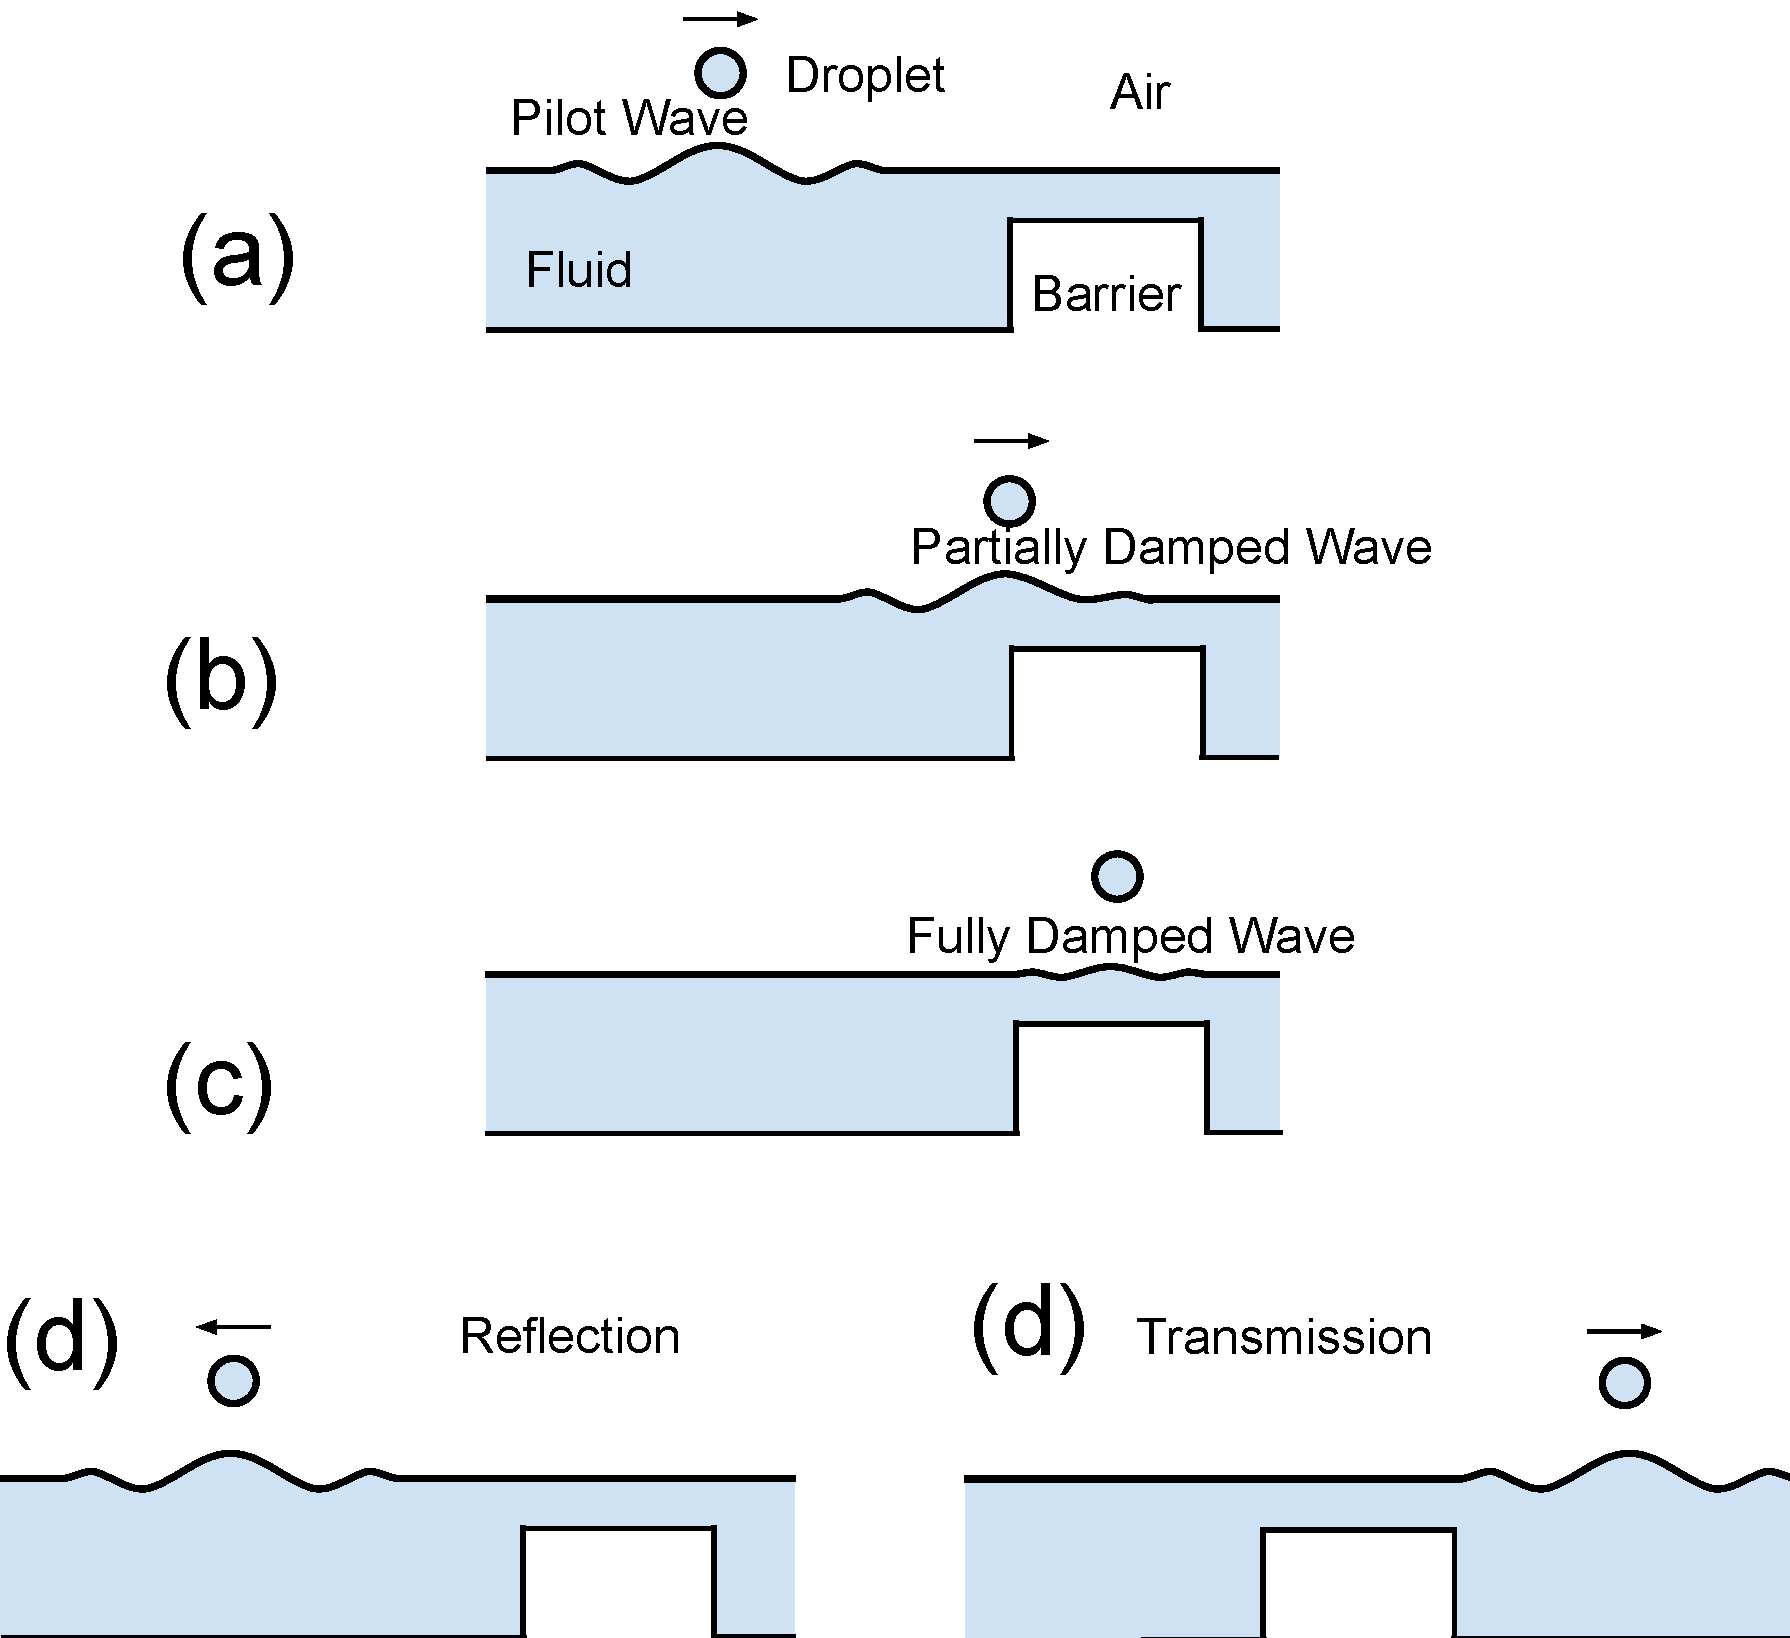
\includegraphics[scale=0.5]{Tunneling}
	     \caption{A diagram of the droplet-barrier interaction. In (a) the droplet moves towards the barrier. As it gets closer (b), the guiding wave is damped. In (c) the guiding wave is fully damped, and then the droplet will either reflect back from where it came (d), or carry on as shown in (e).}
	 \label{tuncartoon}
	\end{figure}
	       The guiding wave field can be partially reflected off of an edge or even a change in depth of the oil bath. This effect can be seen when a walker is pushed back from a under-the-surface step, seemingly without any contact. In rare cases, the walker will actually ``tunnel" across the step; that is, it will continue to walk along the surface of the oil bath and pass over the step without reflection. This interaction is sketched in \refFig{tuncartoon}. In the first experiment done by Eddi et al., they demonstrated tunneling by by building square ``corrals" of varying thicknesses\cite{tunneling}. In the second experiment, they built a rhombus shape which forced the walker across the center of a rhombus. The barrier was placed perpendicular to the direction of travel of the walker, so that it would hit the wall directly rather than at an angle (as in the square corral). ``The tunneling probability decreases exponentially with the barrier width and increases as the Faraday threshold is approached." Eddi et. al also found that the probability of tunneling increased with the velocity of the walker.  The unpredictability of the tunneling comes from the complex interaction between the drop and its guiding wave. 


